\section{Progettazione concettuale}

\subsection{Diagramma Delle Classi UML}

\begin{figure}[ht]
    \centering
    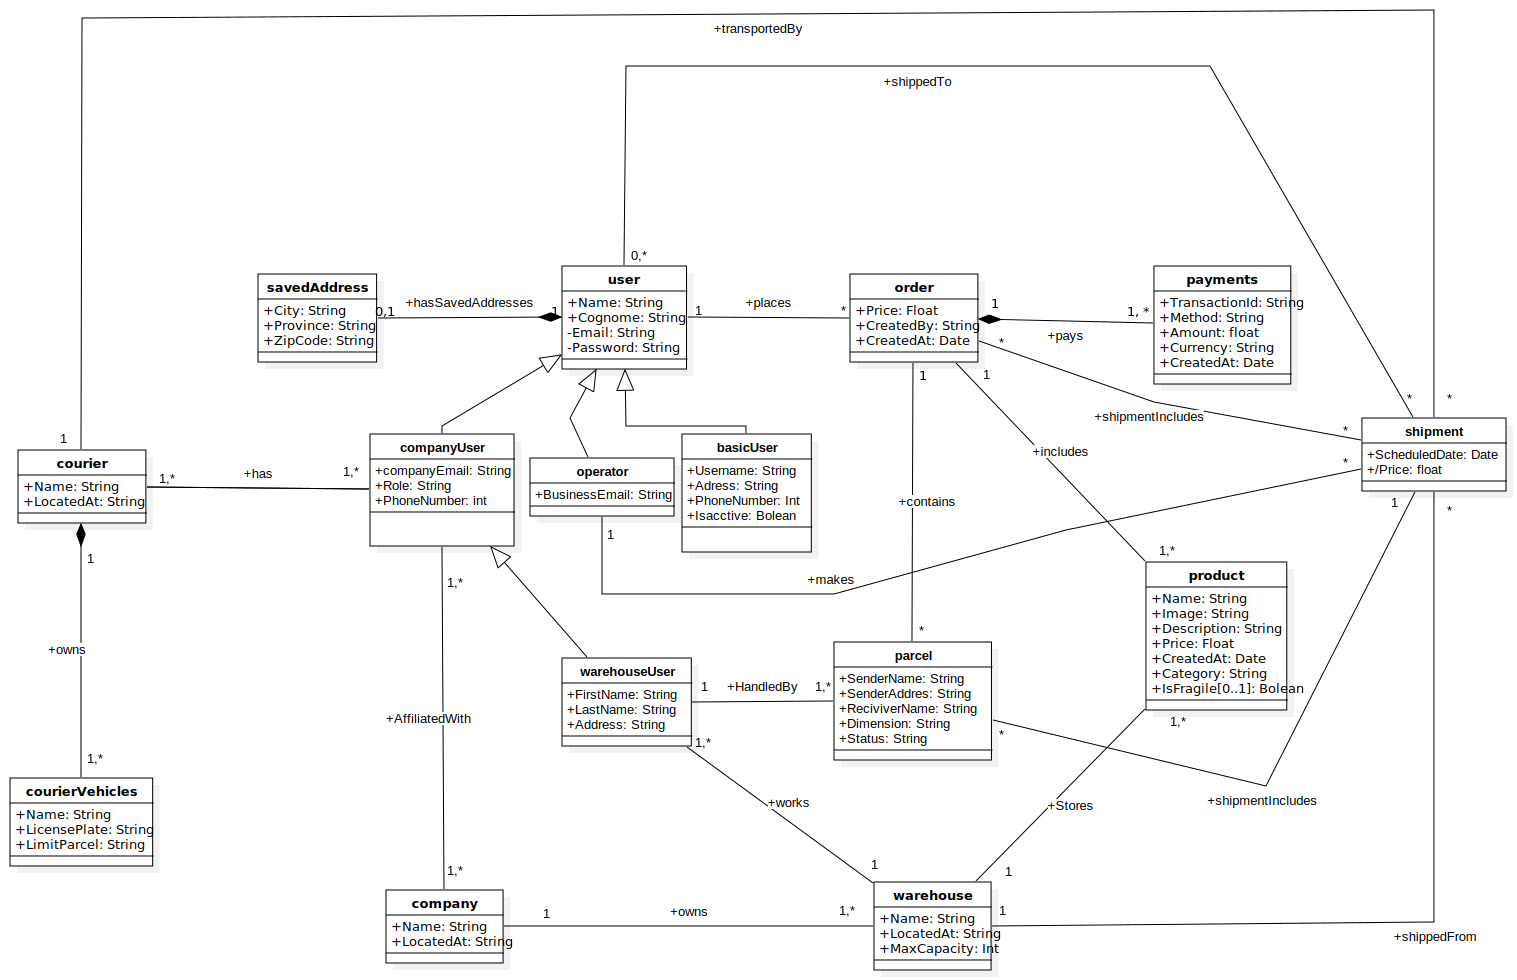
\includegraphics[scale=0.4]{imgs/umlConcettuale.pdf}
    \caption{Diagramma delle classi UML}
\end{figure}

\newpage

\subsection{Leggenda del Diagramma Entità-Relazione}

Nella creazione del diagramma Entità-Relazione, abbiamo impiegato diversi colori per distinguere chiaramente le varie componenti. Per assicurare la chiarezza e facilitare la comprensione del diagramma, di seguito è presentata una leggenda che spiega i simboli usati e i loro colori corrispondenti:
\begin{itemize}[leftmargin=*,label={\textbullet},itemsep=0pt,topsep=0pt,partopsep=0pt]
    \item \textbf{Entità}:
          \begin{itemize}[leftmargin=*,label={\textbullet},itemsep=0pt,topsep=0pt,partopsep=0pt]
            \item \textbf{Rettangolo Azzurro}:  Rappresenta un'entità. Il nome dell'entità è posizionato all'interno del rettangolo;
            \item \textbf{Rettangolo Grigio con doppia linea}: Indica un'entità debole.
          \end{itemize}
    \item \textbf{Attributo}:
          \begin{itemize}[leftmargin=*,label={\textbullet},itemsep=0pt,topsep=0pt,partopsep=0pt]
            \item \textbf{Ovale Giallo}: Rappresenta un attributo. Il nome dell'attributo è posizionato all'interno dell'ovale;
            \item \textbf{Ovale tratteggiato}: Indica un attributo derivato;
            \item \textbf{Nome sottolineato}: Indica un attributo chiave.
          \end{itemize}
    \item \textbf{Relazione}:
          \begin{itemize}[leftmargin=*,label={\textbullet},itemsep=0pt,topsep=0pt,partopsep=0pt]
            \item \textbf{Rombo Verde}: Rappresenta una relazione. Il nome della relazione è posizionato all'interno del rombo;
            \item \textbf{Rombo con Doppia Linea}: Indica una relazione di tipo debole.
          \end{itemize}
    \item \textbf{Specializzazioni}:
          \begin{itemize}[leftmargin=*,label={\textbullet},itemsep=0pt,topsep=0pt,partopsep=0pt]
            \item \textbf{Cerchio e Linea Rosa}: Rappresentano una specializzazione.
                  \begin{itemize}[leftmargin=*,label={\textbullet},itemsep=0pt,topsep=0pt,partopsep=0pt]
                    \item \textbf{Lettera "U" (Magnete)}: Indica la direzione della sottoclasse nella specializzazione;
                    \item \textbf{Lettera "d"}: Specifica una specializzazione disgiunta;
                    \item \textbf{Lettera "o"}: Specifica una specializzazione overlapping;
                    \item \textbf{Singola Linea}: Rappresenta la parzialità della specializzazione;
                    \item \textbf{Doppia Linea}: Rappresenta la totalità della specializzazione.
                  \end{itemize}
          \end{itemize}
\end{itemize}

\newpage

\subsection{Diagramma Entità-Relazione}

\begin{figure}[ht]
    \centering
    \includegraphics[scale=0.29]{imgs/Untitled Workspace.pdf}
    \caption{Diagramma Entità-Relazione}
\end{figure}

\newpage

\section{Ristrutturazione}

\subsection{Considerazioni}

\subsubsection{Attributi Multivalore e Composti}

Durante la fase di progettazione concettuale del database, è stata presa una decisione riguardo agli attributi multivalore e composti. Abbiamo scelto di evitare l'uso di attributi multivalore o composti. Questa decisione è stata guidata dalla necessità di mantenere una struttura di database chiara e di facile gestione.

\subsubsection{Specializzazioni}

Le varie \textbf{specializzazioni} e le varie \textbf{generalizzazioni} sono state modellate nei seguenti modi:

\begin{itemize}[leftmargin=*,label={\textbullet},itemsep=0pt,topsep=0pt,partopsep=0pt]
    \item \textbf{Employee}:
          \begin{itemize}[leftmargin=*,label={\textbullet},itemsep=0pt,topsep=0pt,partopsep=0pt]
            \item \textbf{Tipo di Specializzazione}: Totale e disgiunta;
            \item \textbf{Implementazione}: Abbiamo scelto di accorpare la classe generale \textbf{Employee} in classi specializzate.
          \end{itemize}
    \item \textbf{User}:
          \begin{itemize}[leftmargin=*,label={\textbullet},itemsep=0pt,topsep=0pt,partopsep=0pt]
            \item \textbf{Tipo di Specializzazione}: Parziale e Totale;
            \item \textbf{Implementazione}: Per la specializzazione di \textbf{Account}, abbiamo deciso di trasformarla in un'associazione. Questo approccio ci ha permesso di limitare i vincoli d'integrità e di gestire in modo più efficace i campi che possono assumere valori null.
          \end{itemize}
\end{itemize}

\subsubsection{Attributi Derivati}

Nel contesto della progettazione concettuale del database, abbiamo implementato tre attributi derivati, gestendoli nel seguente modo:

\begin{itemize}[leftmargin=*,label={\textbullet},itemsep=0pt,topsep=0pt,partopsep=0pt]
    \item \textbf{Attributo Price}:
          \begin{itemize}[leftmargin=*,label={\textbullet},itemsep=0pt,topsep=0pt,partopsep=0pt]
            \item \textbf{Gestione}: Nonostante \textbf{Price} sia un attributo derivato (tipicamente calcolato a partire da altri dati), abbiamo deciso di conservarlo direttamente nel nostro sistema.
            \item \textbf{Motivazione}: Questa scelta è stata fatta per ottimizzare le prestazioni del sistema, evitando il calcolo ripetuto dei prezzi ogni volta che vengono richiesti. Conservando il prezzo calcolato, riduciamo il carico sul sistema e miglioriamo l'efficienza delle query.
          \end{itemize}
    \item \textbf{Attributo OccupiedSpace}:
          \begin{itemize}[leftmargin=*,label={\textbullet},itemsep=0pt,topsep=0pt,partopsep=0pt]
            \item \textbf{Gestione}: Abbiamo scelto di conservare anche l'attributo \textbf{OccupiedSpace} all'interno del nostro sistema.
            \item \textbf{Motivazione}: Questa decisione è stata presa considerando l'importanza di questo attributo, che può essere frequentemente richiesto dal sistema per la gestione degli spazi nei magazzini. Conservandolo, siamo in grado di fornire rapidamente le informazioni richieste senza la necessità di calcoli aggiuntivi.
          \end{itemize}
\end{itemize}

\newpage

\subsubsection{Analisi delle Ridondanze}

Nel processo di ottimizzazione del database, abbiamo eseguito un'analisi dettagliata per identificare e risolvere eventuali ridondanze.

\begin{itemize}[leftmargin=*,label={\textbullet},itemsep=0pt,topsep=0pt,partopsep=0pt]
  \item \textbf{Ridondanza negli attributi delle associazioni}:
        \begin{itemize}[leftmargin=*,label={\textbullet},itemsep=0pt,topsep=0pt,partopsep=0pt]
          \item \textbf{Situazione Identificata}: Dopo la ristrutturazione delle specializzazioni, abbiamo riscontrato la presenza di ridondanza negli attributi. In particolare, l'attributo \textbf{BusinessEmail} era presente sia nell'associazione \textbf{Driver} che in \textbf{Operator}, pur essendo associato a due entità diverse.
          \item \textbf{Soluzione Implementata}: Per risolvere questa ridondanza, abbiamo introdotto attributi identificativi specifici per ciascuna associazione. Nell'associazione \textbf{Driver}, è stato aggiunto l'attributo \textbf{driverId} per identificare univocamente ogni driver. Analogamente, nell'associazione \textbf{Operator}, è stato introdotto \textbf{operatorId} per l'identificazione univoca degli operatori.
        \end{itemize}
  \item \textbf{Ambiguità nei nomi delle relazioni}:
        \begin{itemize}[leftmargin=*,label={\textbullet},itemsep=0pt,topsep=0pt,partopsep=0pt]
          \item \textbf{Situazione Identificata}: Abbiamo notato una sovrapposizione nei nomi delle relazioni tra \textbf{Order} e \textbf{Shipment} e tra \textbf{Parcel} e \textbf{Shipment}. Nonostante avessero lo stesso nome, queste relazioni indicavano relazioni sostanzialmente diverse.
          \item \textbf{Soluzione Implementata}: Per eliminare questa ambiguità, abbiamo deciso di rinominare la relazione tra \textbf{Order} e \textbf{Shipment} in \textbf{orderShipment}. Questo aiuta a distinguere chiaramente questa relazione da quella tra \textbf{Parcel} e \textbf{Shipment}.
        \end{itemize}
\end{itemize}

\subsubsection{Identificazione delle Chiavi Primarie}

Abbiamo effettuato delle scelte riguardo all'uso di chiavi primarie, in particolare l'introduzione di chiavi surrogate in alcune associazioni chiave.

\begin{itemize}[leftmargin=*,label={\textbullet},itemsep=0pt,topsep=0pt,partopsep=0pt]
  \item \textbf{Associazione Order}:
        \begin{itemize}[leftmargin=*,label={\textbullet},itemsep=0pt,topsep=0pt,partopsep=0pt]
          \item \textbf{Decisione}: Introduzione di una chiave surrogata per identificare univocamente ogni ordine chiamata \textbf{OrderId}.
          \item \textbf{Motivazione}: L'uso di una chiave surrogata in questa associazione assicura che ogni ordine registrato nel sistema sia univoco. Questo non solo semplifica la gestione e il tracciamento degli ordini attuali, ma apre anche la strada per un potenziale supporto di funzionalità avanzate, come la gestione di ordini multipli o complessi in futuro.
        \end{itemize}
  \item \textbf{Associazioni Driver e Operator}:
        \begin{itemize}[leftmargin=*,label={\textbullet},itemsep=0pt,topsep=0pt,partopsep=0pt]
          \item \textbf{Decisione}: Aggiunta di chiavi surrogate in entrambe le associazioni, come menzionato nell'analisi delle ridondanze.
          \item \textbf{Motivazione}: Questa scelta è stata guidata dall'analisi della ridondanza, garantendo un'identificazione chiara e distinta di ogni driver e ogni operatore.
        \end{itemize}
  \item \textbf{Associazione Company}:
        \begin{itemize}[leftmargin=*,label={\textbullet},itemsep=0pt,topsep=0pt,partopsep=0pt]
          \item \textbf{Decisione}: Introduzione di una chiave surrogata nell'associazione \textbf{Company}, chiamata \textbf{CompanyId}.
          \item \textbf{Motivazione}: Abbiamo identificato la necessità di un identificatore unico più affidabile del solo nome aziendale, avendo riscontrato casi di aziende con lo stesso nome. La chiave surrogata assicura una distinzione precisa tra le aziende, anche in presenza di nomi omonimi.
        \end{itemize}
\end{itemize}